\documentclass[12pt,letterpaper]{article}

% Librerías a utilizar
\usepackage[utf8]{inputenc}	% Codificación 
\usepackage[spanish]{babel}	% Idioma
\usepackage{natbib}			% Bibliografía
\usepackage{graphicx}		% Imagenes
\usepackage{indentfirst}		% Sangría
\usepackage{amsmath, amsfonts, amssymb}	% Figuras matemáticas
\usepackage{url}							% URL
\usepackage{listings}
\usepackage{subcaption}

\lstset{language=Python,
	basicstyle={\small\ttfamily}	
}

\usepackage[left=3cm,right=2cm,top=2cm,bottom=3cm]{geometry}

\setlength{\parindent}{2cm}	% Sangría en los párrafos
\renewcommand{\baselinestretch}{1.5}	% Interlineado

% Renombrar ciertos títulos del texto
\renewcommand\spanishcontentsname{Tabla de contenidos}
\renewcommand\spanishrefname{Bibliografía}

% Inicio del documento
\begin{document}

%%%%%%%%% PORTADA %%%%%%%%%

\newpage
\vspace*{-.5cm}
% Logo institucional
\begin{picture}(18,4)(0,30)
	\put(350,-20){\includegraphics[scale=0.25]{./images/LogoUsach.pdf}}
\end{picture}

\sloppy
\thispagestyle{empty}
\vspace*{-1.6cm}

% Datos institucionales
\begin{center}
	{\bf \mbox{\large UNIVERSIDAD DE SANTIAGO DE CHILE}}\\
	{\bf \mbox{FACULTAD DE INGENIER\'IA}}\\
	{\bf \mbox{DEPARTAMENTO DE INGENIER\'IA INFORM\'ATICA}}\\
\end{center}

	\vspace{5cm}
	%Título del trabajo
	\begin{center}
	\Large
		\textbf{Informe de Estado de Avance}
	\end{center}
	
	% Datos personales
	\vspace*{5.5cm}
	\begin{flushright}
        \begin{footnotesize}
        \begin{tabular}[H]{p{5cm} p{8cm}}
            Título del tema: & Reconocimiento de patologías bucales por medio de modelos de aprendizaje profundo\\
			Profesor guía: & Gonzalo Acuña\\
            Fecha de inscripción del tema: & 08 de Octubre de 2020\\
            Alumno: & Daniel Cristobal Labra Leyton \\
            Carrera: & Ingeniería de ejecución en computación e informática\\
            Fecha de egreso: & 26 de Septiembre de 2020\\
            Fecha de entrega del informe: & 20 de Agosto de 2021\\

		\end{tabular}
        \end{footnotesize}
	\end{flushright}
	\begin{center}
		\vspace{1.5cm}
		% Fecha
		\Today
	\end{center}

\newpage
\tableofcontents
\thispagestyle{empty}

\newpage
\renewcommand{\thepage}{\arabic{page}}
\setcounter{page}{1}

% Capítulos agregados 
\section{Objetivo general del proyecto}
El objetivo general del proyecto es implementar un modelo de aprendizaje profundo para el reconocimiento de patologías bucales comunes, a través de fotografías digitales de la cavidad bucal de las personas.

%\subsection{Objetivos Especificos:}
%\begin{enumerate}
%	\item Investigar sobre la herramienta de simulacion Robóticos CoppeliaSim y su integración con API's para implementación de código de control.
%	\item Implementar en CoppeliaSim un entorno de simulación con un manipulador Robótico a elección y una correa tranportadora de cubos.
%	\item Implementar control manual y automático desde una interfaz desarrollada por nosotros para esolver un problema de apilamiento de objetos.
%\end{enumerate}

\section{Estado de avance}
A continuación se presenta el último plan de trabajo informado al departamento.

\begin{figure}[!ht]
    \centering
    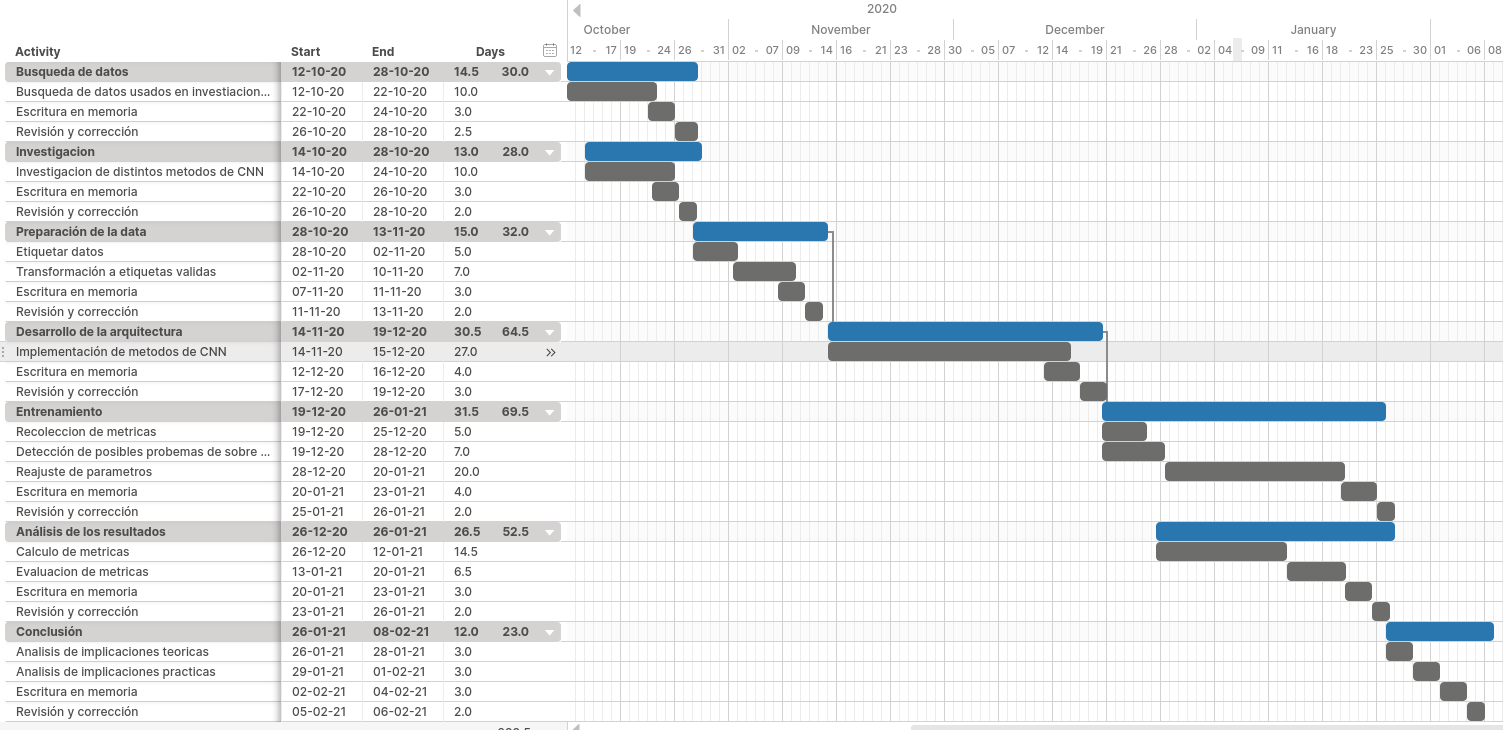
\includegraphics[scale=0.457]{images/planTrabajo.png}
    \caption{Plan de trabajo original}
    \label{fig:planTrabajo}
\end{figure}

De este plan de trabajo las actividades búsqueda de datos, investigación, preparación de la data, desarrollo de la arquitectura y entrenamiento se han realizado, sin embargo, los resultados obtenidos en la fase de entrenamiento indican que los datos recopilados para entrenar el modelo son insuficientes aún, por lo que en este momento se esta realizando data augmentation e incluso se ha implementado una red neuronal GAN para crear data artificial ya que la que se tiene presenta grandes desbalances entre clases, es por esta razón que se necesita más tiempo para completar el trabajo.

\section{Nuevo plan de trabajo}
A continuación se presenta la nueva propuesta de plan de trabajo donde se considera la etapa de data augmentation y el entrenamiento de la nueva data obtenida, además de las etapas faltantes.

\begin{figure}[!ht]
    \centering
    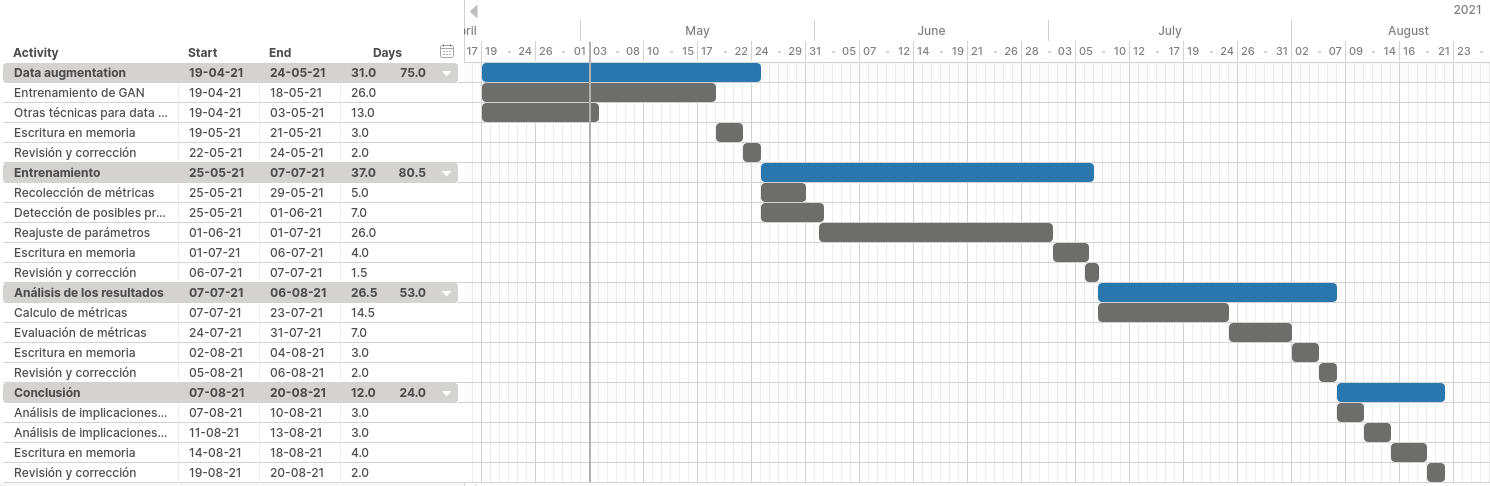
\includegraphics[scale=0.458]{images/newPlan.png}
    \caption{Nuevo plan de trabajo propuesto}
    \label{fig:newPlan}
\end{figure}

\begin{figure}[!bt]
    \centering
    
\includegraphics[scale=0.3]{images/firma2.png}
    \caption{Firma profesor guia}
    \label{fig:firma}
\end{figure}

\begin{figure}[!bt]
    \centering
    
\includegraphics[scale=0.6]{images/miFirma.png}
    \caption{Firma alumno}
    \label{Fig:miFirma}
\end{figure}

%\subsection{Datos}
%\begin{itemize}
%	\item Dato 1
%	\item Dato 2
%	\item Dato 3
%\end{itemize}


\clearpage
%\addcontentsline{toc}{section}{Bibliografía}
%\bibliographystyle{apalike}
%\bibliography{bibliografia}

\end{document}
